\section{Results}
\label{sec:results}

The final topology optimization results are shown in Figures \ref{fig:optimized_results} and \ref{fig:smoothed_results}.

\begin{figure}[H]
    \centering
    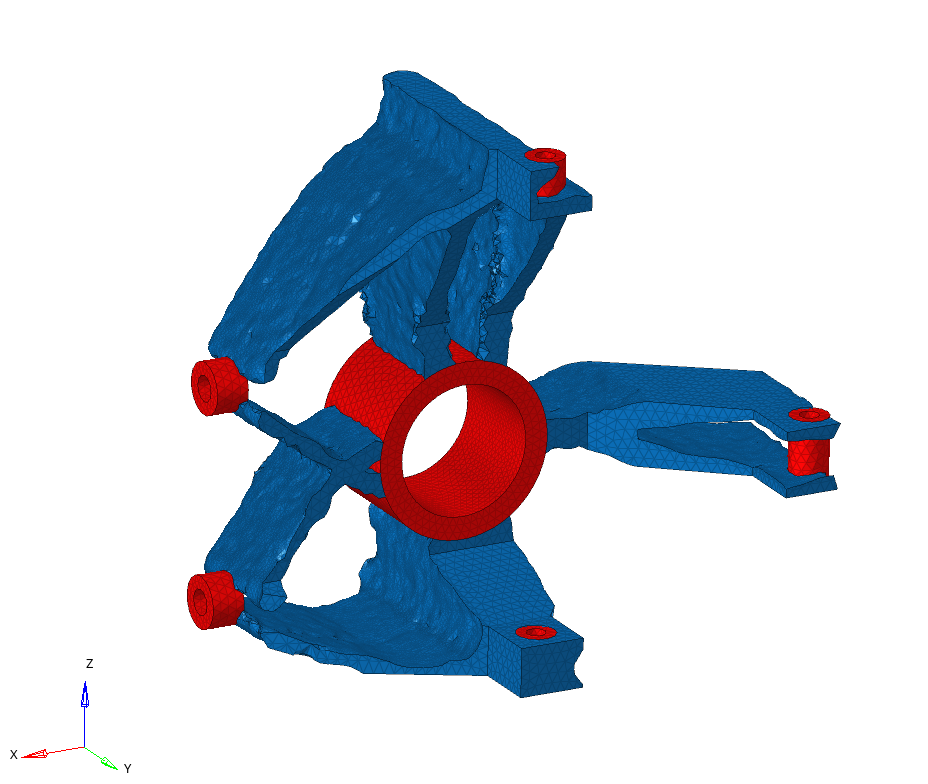
\includegraphics[width=0.8\textwidth]{img/optimized_design_domain.png}
    \caption{Optimized design.}
    \label{fig:optimized_results}
\end{figure}

\begin{figure}[H]
    \centering
    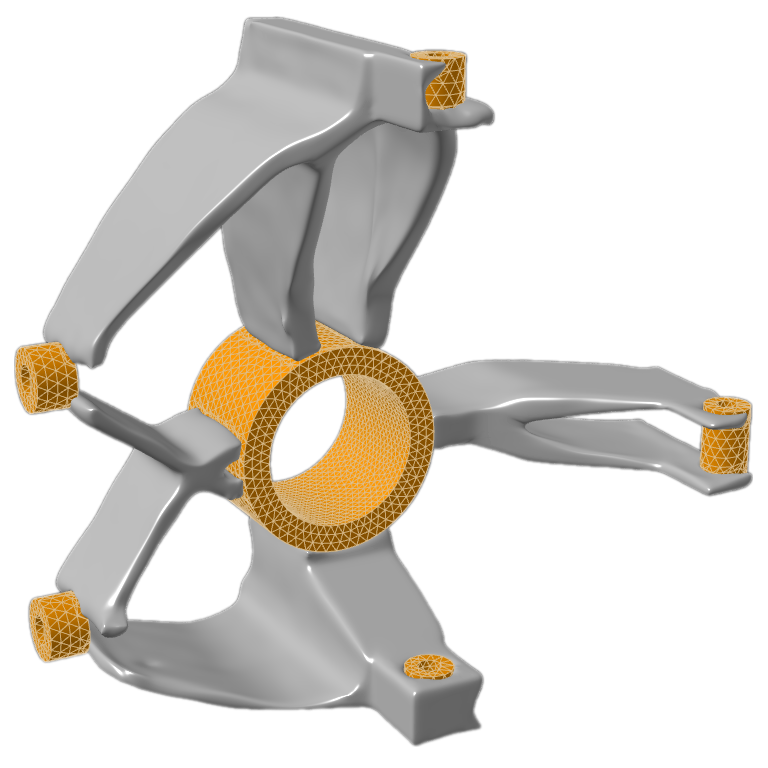
\includegraphics[width=0.48\textwidth]{img/smoothed_design_domain_front_no_bg.png}
    \hfill
    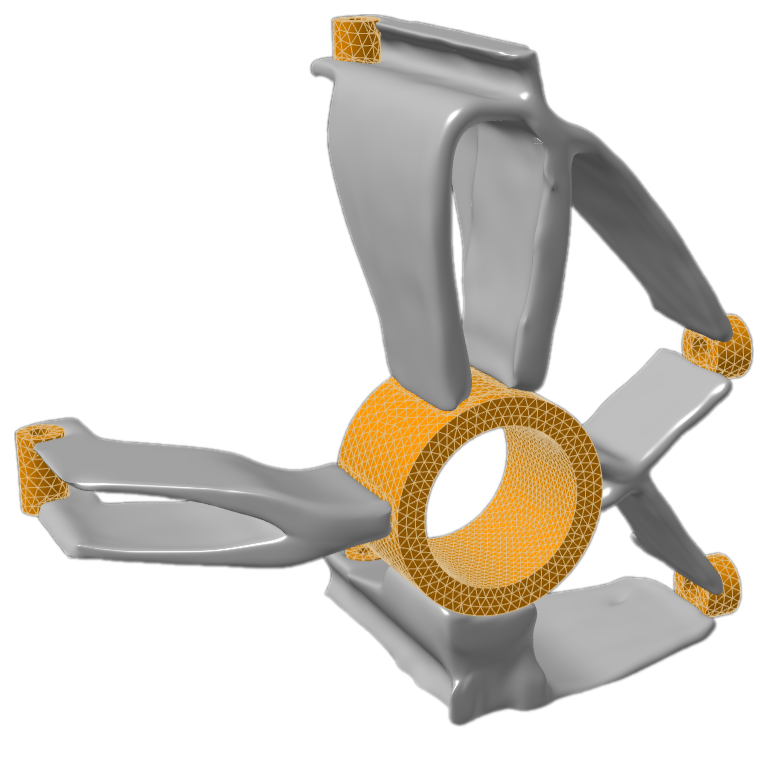
\includegraphics[width=0.48\textwidth]{img/smoothed_design_domain_rear_no_bg.png}
    \caption{Smoothed design.}
    \label{fig:smoothed_results}
\end{figure}

Due to limitation in the number of elements imposed by the student version of the software, the meshing element has been chosen to be tetrahedral with a size of $3.0 [mm]$ on both the design and non-design domain.

The optimization process converged after $47$ iterations with a final weighted compliance of $224.15[J]$ and a final mass of $0.45[kg]$ (initial mass was $1.98[kg]$).
Both the constraints imposed on the stiffness are respected (stiffness computed as the inverse of the maximum rotation at point $A$ in presence of a unitary moment):

\begin{itemize}
    \item Camber stiffness: $K_c = 1 / 6.26 \cdot 10^{-6} [Nm / rad] = 159.7 \cdot 10^3 [Nm/rad]$;
    \item Toe stiffness: $K_t = 1 / 1.14 \cdot 10^{-5} [Nm / rad] = 87.7 \cdot 10^3 [Nm/rad]$.
\end{itemize}

Given the imposed high stiffness constraints, we can expect that also the dissipation of energy from the vehicle due to out-of-plane deformations will be minimized, thus improving the overall vehicle performance.


\subsection{Finite Element Analysis}
\label{subsec:finite_element_analysis}

The final design has been analyzed using a Finite Element Analysis (FEA) to verify the stiffness and the stress distribution.
The results are shown in the following figures.

From Von Mises stress distribution, it is possible to observe that the hotspots is located at the interface between the lower control arm and the main body of the hub carrier.
Moreover, the most stressed condition appears to be the braking load cases, with a maximum stress of $37.4 [MPa]$ which is below the yield strength of the material.

For deformations, a scale factor of $500$ has been applied in order to better visualization.

\begin{figure}[H]
    \centering
    
\includegraphics[width=0.49\textwidth]{img/fem/pure_rolling.png}
    \hfill
    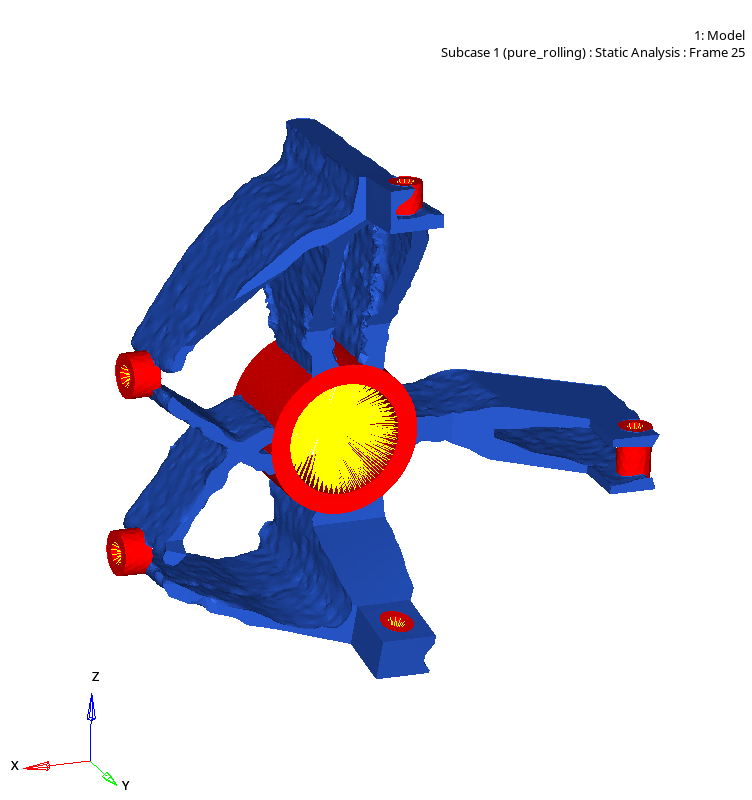
\includegraphics[width=0.49\textwidth]{img/displacements/pure_rolling.png}
    \caption{Pure rolling.}
\end{figure}

\begin{figure}[H]
    \centering
    
\includegraphics[width=0.49\textwidth]{img/fem/braking.png}
    \hfill
    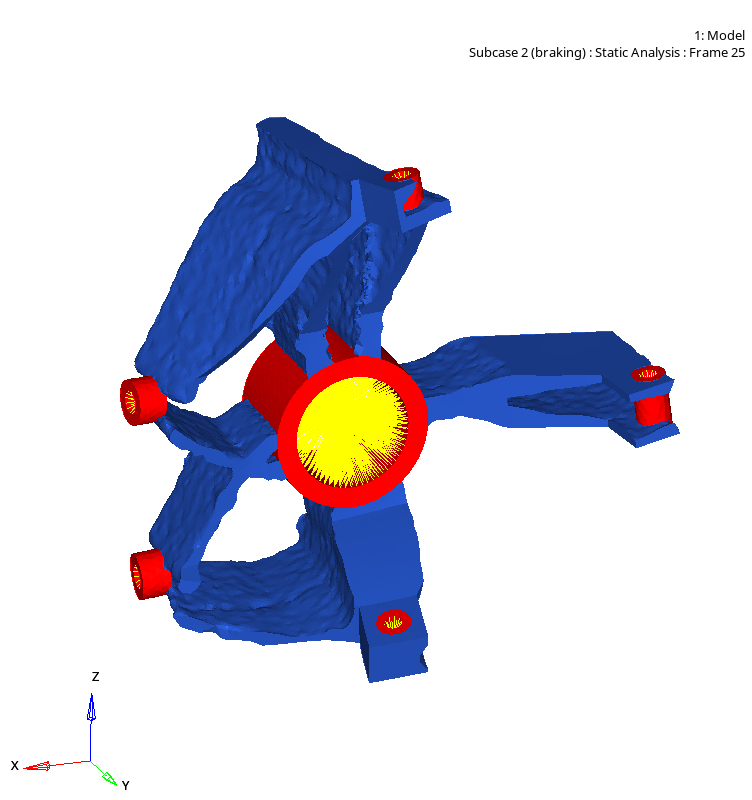
\includegraphics[width=0.49\textwidth]{img/displacements/braking.png}
    \caption{Braking.}
\end{figure}

\begin{figure}[H]
    \centering
    
\includegraphics[width=0.49\textwidth]{img/fem/internal_turn.png}
    \hfill
    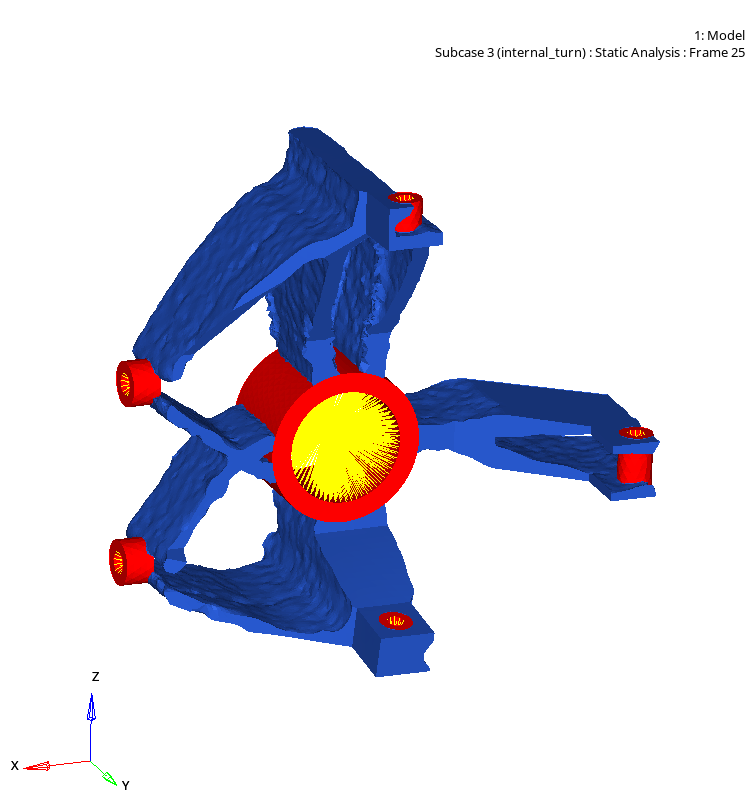
\includegraphics[width=0.49\textwidth]{img/displacements/internal_turn.png}
    \caption{Internal turn.}
\end{figure}

\begin{figure}[H]
    \centering
    
\includegraphics[width=0.49\textwidth]{img/fem/external_turn.png}
    \hfill
    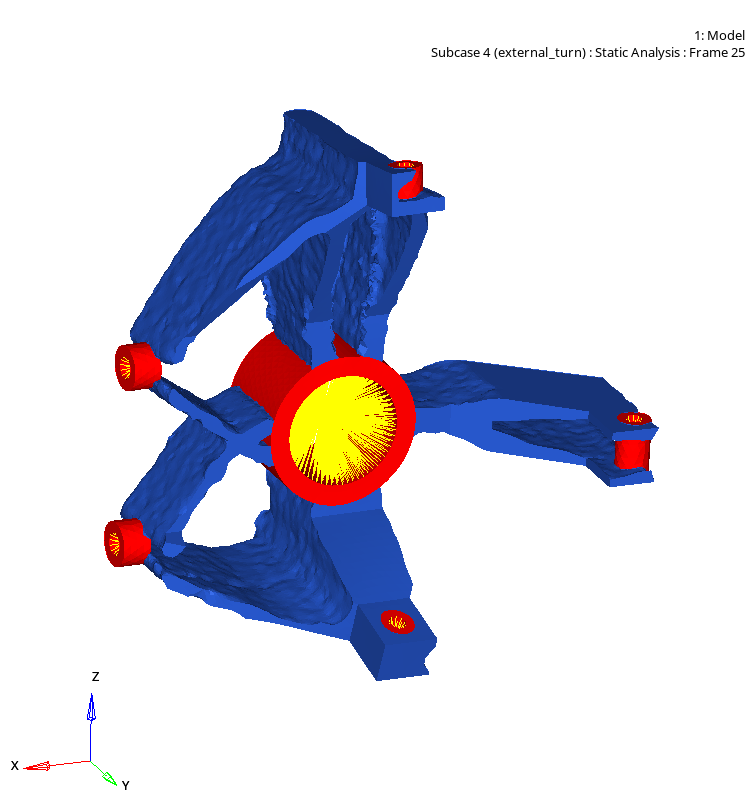
\includegraphics[width=0.49\textwidth]{img/displacements/external_turn.png}
    \caption{External turn.}
\end{figure}

\begin{figure}[H]
    \centering
    
\includegraphics[width=0.49\textwidth]{img/fem/internal_obstacle.png}
    \hfill
    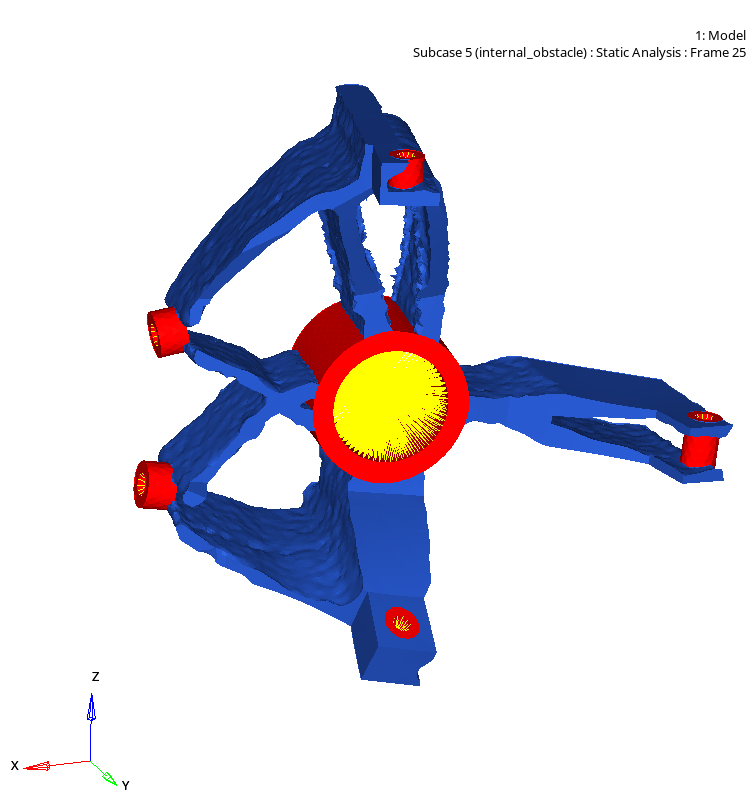
\includegraphics[width=0.49\textwidth]{img/displacements/internal_obstacle.png}
    \caption{Internal obstacle.}
\end{figure}

\begin{figure}[H]
    \centering
    
\includegraphics[width=0.49\textwidth]{img/fem/external_obstacle.png}
    \hfill
    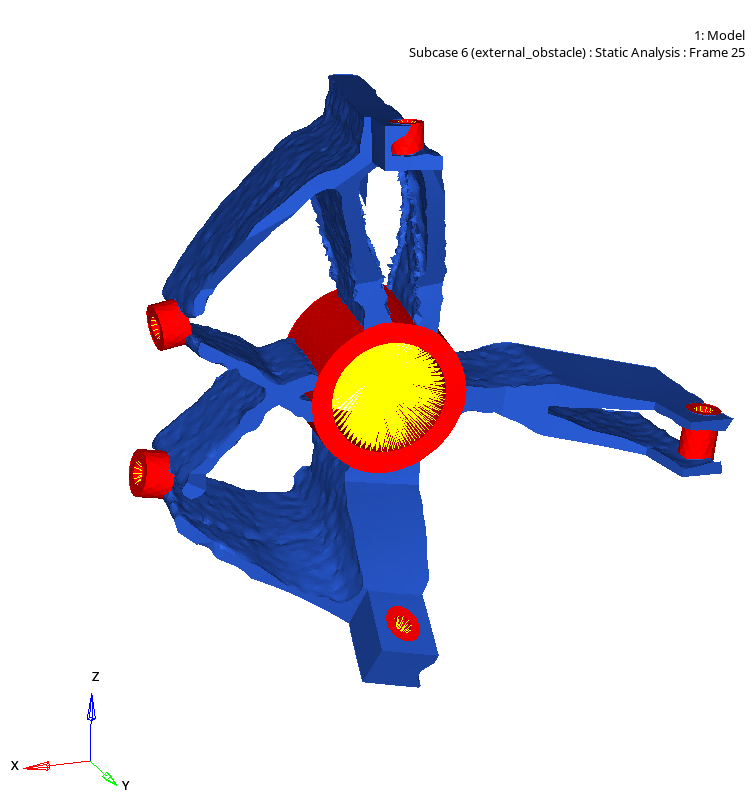
\includegraphics[width=0.49\textwidth]{img/displacements/external_obstacle.png}
    \caption{External obstacle.}
\end{figure}

